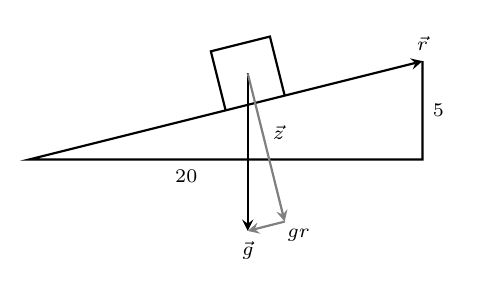
\begin{tikzpicture}[>=stealth]
	\begin{scope}[scale=.25]
			\draw [thick,->] (20,5) -- node [right,pos=.5] {\scriptsize $5$} (20,0) -- node [below,pos=.6] {\scriptsize 20}(0,0) -- (20,5) node [above] {\scriptsize $\vec r$};
			\draw [thick] (10,2.5) -- (9.25,5.5) -- (12.25,6.25) -- (13,3.25);
			\draw [thick,->] (11.125,4.375) -- (11.125,-3.625) node [below] {\scriptsize $\vec g$};
			\draw [gray,thick,->] (11.125,4.375) -- (13,-3.15) node [right,pos=.4,black] {\scriptsize $\vec z$};
			\draw [gray,thick,->] (13,-3.15) -- (11.125,-3.625)node [shift={(5pt,-5pt)} ,black,pos=0] {\scriptsize $\proj gr$};
	\end{scope}

\end{tikzpicture}
